\documentclass{beamer}
%
% Choose how your presentation looks.
%
% For more themes, color themes and font themes, see:
% http://deic.uab.es/~iblanes/beamer_gallery/index_by_theme.html
%
\mode<presentation>
{
  \usetheme{Warsaw}      % or try Darmstadt, Madrid, Warsaw, ...
  \usecolortheme{default} % or try albatross, beaver, crane, ...
  \usefonttheme{default}  % or try serif, structurebold, ...
  \setbeamertemplate{navigation symbols}{}
  \setbeamertemplate{caption}[numbered]
}
\usepackage[L7x]{fontenc}
\usepackage{caption}
\usepackage{lmodern} 
%%%%movie%%%
\setbeamertemplate{itemize items}[circle]

%%%%%%%%%%%%%%%%%%%%%5
\usepackage{multimedia}
\usepackage{animate}

\usepackage{envmath}
%\usepackage{amsmath,amssymb}
\usepackage{cancel}
\usepackage{graphicx}
\usepackage{epsfig}
\usepackage{amsmath,amsfonts,amssymb}
\usepackage{natbib}

\usepackage[T1]{fontenc}
\usepackage[english]{babel}
\usepackage{hyphenat}
\hyphenation{mate-mática recu-perar}
\bibliographystyle{unsrtnat}
\usepackage{tabularx} % extra features for tabular environment
\usepackage{amsmath}  % improve math presentation
\usepackage{blindtext}
%\usepackage{enumitem} tirar isto no beamer
\usepackage{xcolor}
\usepackage{graphicx} % takes care of graphic including machinery
\usepackage{graphics} 
\usepackage{float}
%\usepackage[margin=1in,letterpaper]{geometry}% decreases margins
%\usepackage{cite} % takes care of citations

\usepackage{lipsum}
\usepackage{mwe}
 \newcommand{\sign}{\mathop{\mathrm{sign}}}

\graphicspath{{images/}}
\usepackage{cases}

%%%%%%%%%%%%%%%%%%%%%%%%5

\usepackage[english]{babel}
\usepackage[utf8x]{inputenc}

\title[PMEFT]{Control of a Robotic Leg for Walking, Running and Hopping in Irregular Surfaces}
\author{Author: Nuno Teixeira nº 75494 \\ Supervisor: Rui Dilão}

%\author[Candidate]{Nuno Teixeira nº 75494}
%\author[Supervisor]{Rui Dilão}
%\author[Nuno Teixeira]{Nuno Teixeira\\[10mm]{\small Supervisors: Rui Dilão}}}
%\author[author1]{Nuno Teixeira\\[2mm]{\small Supervisors: Rui Dilão}}
\institute{Projecto MEFT \\Instituto Superior Técnico}
\titlegraphic{
\includegraphics[width=10cm]{logos.png}}
\date{\today}
\setbeamersize{text margin left=0.5cm,text margin right=0.5cm}


\addtolength{\headsep}{0.6cm}


\begin{document}

\begin{frame}
  \titlepage
\end{frame}

\section{No knee models}
\subsection{Running/hopping}
\centering
\begin{frame}{Running and hopping model}
  \centering
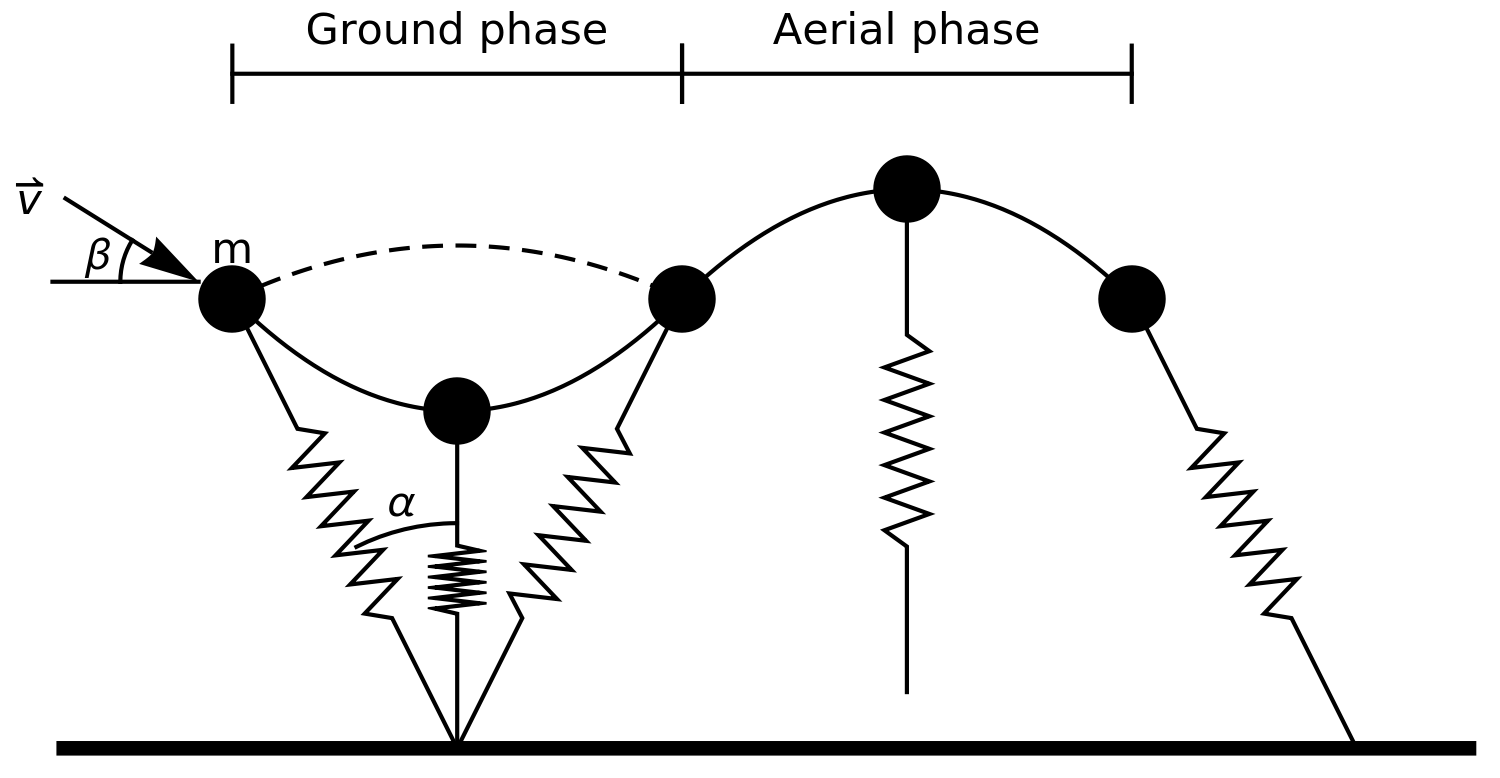
\includegraphics[width=0.8\textwidth]{Blickhan_model.png}
\end{frame}

\begin{frame}{Equations}
  \begin{block}{Ground phase}
  \begin{equation}
  \ddot{x}=x\omega^2\left(\frac{l}{\sqrt{x^2+y^2}}-1\right),
\end{equation}
\begin{equation}
  \ddot{y}=y\omega^2\left(\frac{l}{\sqrt{x^2+y^2}}-1\right)-g,
\end{equation}
\end{block}

\begin{block}{Aerial phase}
\begin{equation}
  \ddot{x}=0,
\end{equation}
\begin{equation}
  \ddot{y}=-g.
  \end{equation}
\end{block}
with $\omega=\sqrt{k/m}$, the natural frequency of the spring
\end{frame}
\subsection{Walking model}
\begin{frame}{Walking model}
  \begin{center}
  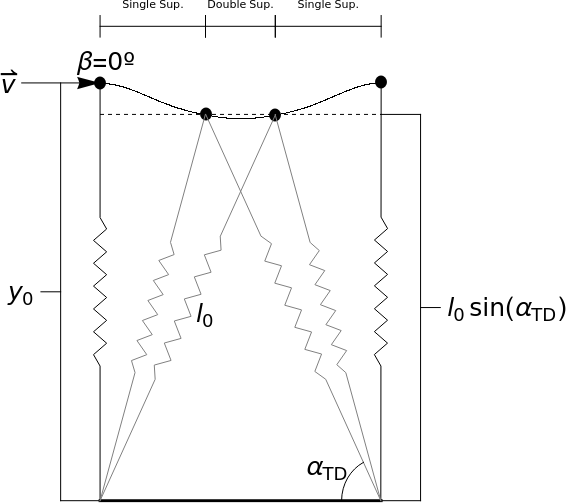
\includegraphics[height=0.5\textheight]{Seyfarth2006_trimmed.png}
  \end{center}
Definitions:
  \begin{itemize}
\item  \underline{stride} - Leg crosses the vertical leg orientation
\item  \underline{step} -The moment when the system passes from single support to double support.
  \end{itemize}
\end{frame}

\begin{frame}{Equations}

  \begin{block}{Single support}
  \begin{equation}
  \ddot{x}=\frac{F_1}{m}\frac{x-x_{t1}}{l_1}
  \label{eq.singlesuppx}
  \end{equation}
\begin{equation}
  \ddot{y}=\frac{F_1}{m}\frac{y-y_{t1}}{l_1}-g
  \label{eq.singlesuppy}
\end{equation}
\end{block}

  \begin{block}{Double support}
\begin{equation}
 \ddot{x}=\frac{F_1}{m}\frac{x-x_{t1}}{l_1}+\frac{F_2}{m}\frac{x-x_{t2}}{l_2}
 \label{eq.doublesuppx}
  \end{equation}
\begin{equation}
  \ddot{y}=\frac{F_1}{m}\frac{y-y_{t1}}{l_1}+\frac{F_2}{m}\frac{y-y_{t2}}{l_2}-g
  \label{eq.doublesuppy}
\end{equation}
\end{block}

\end{frame}

\begin{frame}

with $F_i$ being the force applied on the mass by the respective leg,
\begin{equation}
  F_i=k(l_0-l_i)\geq 0 \,\,\,\,\, i=1,2\,,
\end{equation}
$l_0$ is the natural length of the spring, $l_i$ is the respective length,
\begin{equation}
l_i=\sqrt{(x-x_{ti})^2+(y-y_{ti})^2} \,\,\,\,\, i =1,2 \,.
\end{equation}

Since the system is energetically conservative we can change the initial velocity by inverting
  \begin{equation}
  E=\frac{k (l_0-y_0)^2}{2} + m g y_0 + m \frac{v_0^2}{2}.
\end{equation}

\end{frame}


\begin{frame}{Parameters}

    \begin{block}{A scan is made with 3 parameters, $Energy$, $y_0$, $\alpha$ in two strides}
    \begin{itemize}
\item $Energy \in  [800,840]$ with 40 subdivisions.

\item  $\alpha \in [\pi/2-\pi/5,\pi/2]$ with 30 subdivisions.

\item  $y_0 \in [l_0\sin(\alpha) ,l_0]$ with 25 subdivisions
    \end{itemize}
\end{block}
  In all simulations the following parameters remained fixed.
  \begin{itemize}
    
\item $\beta=0$
  
\item  $m=80 Kg$
  
\item $l_0=1 m$

\item  $k=14000$

 \end{itemize}

Total number of configurations= $40 \times 30 \times 25 = 30000$

 
\end{frame}




\begin{frame}{Survival step configurations}
  Out of the 30000 configurations in the parameter space, only 8195 were able to complete 2 strides. Of this subset of points, 11 fixed points were found, 5 stable and 6 unstable.
  
  From here a survival test is applied to each of the 8195 configurations that completed 2 strides by incrementing steps instead of strides.

  If the simulation fails, the maximum number of steps was assigned to that configuration.
\end{frame}

\begin{frame}{Fixed points and 10 step configurations}
  Iterating the number of steps where $\Delta t=0.00075$ so that in maximum it was possible to achieve 10 steps, the configurations that achieve 10 steps can be ilustrated in the figure below along with the fixed points.
  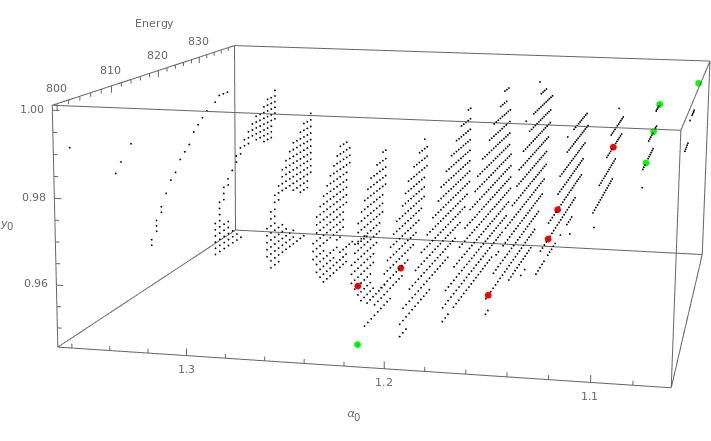
\includegraphics[width=0.8\textwidth]{newfixedpoints.png}


\end{frame}
\section{One knee model}
\subsection{Running/hopping}
\begin{frame}{Running and hopping model - One knee}
  \centering
    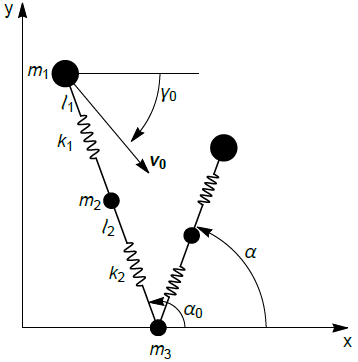
\includegraphics[width=0.6\textwidth]{initialphase.png}
\end{frame}

\begin{frame}{Running and hopping model - One knee}
  \centering
    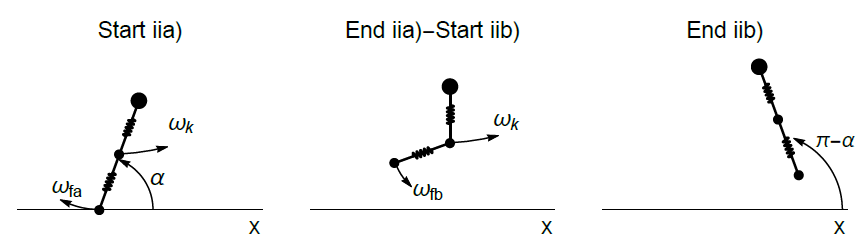
\includegraphics[width=0.8\textwidth]{secondphase.png}
\end{frame}

\begin{frame}{Running and hopping model - One knee}
  \centering
    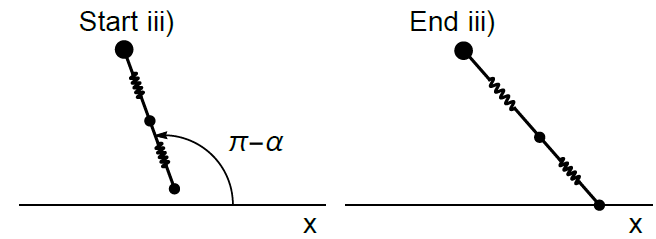
\includegraphics[width=0.8\textwidth]{thirdphase.png}
\end{frame}

\section{Summary}


\end{document}
